\documentclass{article}\usepackage[]{graphicx}\usepackage[]{color}
% maxwidth is the original width if it is less than linewidth
% otherwise use linewidth (to make sure the graphics do not exceed the margin)
\makeatletter
\def\maxwidth{ %
  \ifdim\Gin@nat@width>\linewidth
    \linewidth
  \else
    \Gin@nat@width
  \fi
}
\makeatother

\definecolor{fgcolor}{rgb}{0.345, 0.345, 0.345}
\newcommand{\hlnum}[1]{\textcolor[rgb]{0.686,0.059,0.569}{#1}}%
\newcommand{\hlstr}[1]{\textcolor[rgb]{0.192,0.494,0.8}{#1}}%
\newcommand{\hlcom}[1]{\textcolor[rgb]{0.678,0.584,0.686}{\textit{#1}}}%
\newcommand{\hlopt}[1]{\textcolor[rgb]{0,0,0}{#1}}%
\newcommand{\hlstd}[1]{\textcolor[rgb]{0.345,0.345,0.345}{#1}}%
\newcommand{\hlkwa}[1]{\textcolor[rgb]{0.161,0.373,0.58}{\textbf{#1}}}%
\newcommand{\hlkwb}[1]{\textcolor[rgb]{0.69,0.353,0.396}{#1}}%
\newcommand{\hlkwc}[1]{\textcolor[rgb]{0.333,0.667,0.333}{#1}}%
\newcommand{\hlkwd}[1]{\textcolor[rgb]{0.737,0.353,0.396}{\textbf{#1}}}%
\let\hlipl\hlkwb

\usepackage{framed}
\makeatletter
\newenvironment{kframe}{%
 \def\at@end@of@kframe{}%
 \ifinner\ifhmode%
  \def\at@end@of@kframe{\end{minipage}}%
  \begin{minipage}{\columnwidth}%
 \fi\fi%
 \def\FrameCommand##1{\hskip\@totalleftmargin \hskip-\fboxsep
 \colorbox{shadecolor}{##1}\hskip-\fboxsep
     % There is no \\@totalrightmargin, so:
     \hskip-\linewidth \hskip-\@totalleftmargin \hskip\columnwidth}%
 \MakeFramed {\advance\hsize-\width
   \@totalleftmargin\z@ \linewidth\hsize
   \@setminipage}}%
 {\par\unskip\endMakeFramed%
 \at@end@of@kframe}
\makeatother

\definecolor{shadecolor}{rgb}{.97, .97, .97}
\definecolor{messagecolor}{rgb}{0, 0, 0}
\definecolor{warningcolor}{rgb}{1, 0, 1}
\definecolor{errorcolor}{rgb}{1, 0, 0}
\newenvironment{knitrout}{}{} % an empty environment to be redefined in TeX

\usepackage{alltt}[12pt]
\usepackage{Sweave}
\usepackage{float}
\usepackage{graphicx}
\usepackage{tabularx}
\usepackage{siunitx}
\usepackage{amssymb} % for math symbols
\usepackage{amsmath} % for aligning equations
\usepackage{mdframed}
\usepackage{natbib}
\bibliographystyle{..//bib/styles/gcb}
\usepackage[hyphens]{url}
\usepackage[small]{caption}
\setlength{\captionmargin}{30pt}
\setlength{\abovecaptionskip}{0pt}
\setlength{\belowcaptionskip}{10pt}
\topmargin -1.5cm        
\oddsidemargin -0.04cm   
\evensidemargin -0.04cm
\textwidth 16.59cm
\textheight 21.94cm 
%\pagestyle{empty} %comment if want page numbers
\parskip 7.2pt
\renewcommand{\baselinestretch}{2}
\parindent 0pt
\usepackage{lineno}
\linenumbers
\usepackage{setspace}
\doublespacing

\newmdenv[
  topline=true,
  bottomline=true,
  skipabove=\topsep,
  skipbelow=\topsep
]{siderules}

%% R Script


\IfFileExists{upquote.sty}{\usepackage{upquote}}{}
\begin{document}
\noindent 
\textbf{\LARGE{Climate change reshapes the drivers of false spring risk across European trees}} 
%\\
%OR \\
%\textbf{\Large{Climate change increases the risk of false springs in European trees}} \\ % Lizzie votes for the first title! Reviewers can ask you to make it more narrow so I would start here and shift to Ben's if requested ... (goal 1: get paper out for review)
%\textbf{\Large{False spring risk increases across European trees in the face of climate change}}


\noindent Authors:\\
C. J. Chamberlain $^{1,2}$, B. I. Cook $^{3}$, I. Morales-Castilla $^{4,5}$ \& E. M. Wolkovich $^{1,2,6}$
\vspace{2ex}\\
\emph{Author affiliations:}\\
$^{1}$Arnold Arboretum of Harvard University, 1300 Centre Street, Boston, Massachusetts, USA; \\
$^{2}$Organismic \& Evolutionary Biology, Harvard University, 26 Oxford Street, Cambridge, Massachusetts, USA; \\
$^{3}$NASA Goddard Institute for Space Studies, New York, New York, USA; \\
$^{4}$GloCEE - Global Change Ecology and Evolution Group, Department of Life Sciences, Universidad de Alcal\'{a}, Alcal\'{a} de Henares, 28805, Spain \\
$^{5}$Department of Environmental Science and Policy, George Mason University, Fairfax, VA 22030; \\
$^{6}$Forest \& Conservation Sciences, Faculty of Forestry, University of British Columbia, 2424 Main Mall, Vancouver, BC V6T 1Z4\\
\vspace{2ex}
$^*$Corresponding author: 248.953.0189; cchamberlain@g.harvard.edu\\

\renewcommand{\thetable}{\arabic{table}}
\renewcommand{\thefigure}{\arabic{figure}}
\renewcommand{\labelitemi}{$-$}
\setkeys{Gin}{width=0.8\textwidth}

%%%%%%%%%%%%%%%%%%%%%%%%%%%%%%%%%%%%%%%%%%%%%%%
%%%%%%%%%%%%%%%%%%%%%%%%%%%%%%%%%%%%%%%%%%%%%%%

\section*{Abstract}
Temperate and boreal forests are at risk of late spring freezing events---also known as false springs. Research to date has generated conflicting results of whether climate change will decrease false springs, and thus reshape a fundamental factor that shapes species' ranges. Conflicting results may be due to the myriad spatial and environmental factors that contribute to a plants risk of a false spring, which---to date---no study has compared at once. Here, we assessed the effects of the North Atlantic Oscillation (NAO), mean spring temperature, elevation and distance from the coast, using PEP725 leafout data for six tree species across 11,648 sites in Europe, to determine which were the strongest predictors of false spring risk and how these predictors shifted with climate change. False spring risk varied across the six species but, generally, false spring risk is increasing with climate change for early-leafout species and remaining the same or decreasing with late-leafout species. Across species, mean spring temperature and distance from the coast were the strongest predictors of false spring risk, with higher mean spring temperatures having fewer false springs (-7.6\% for every 2$^{\circ}$C increase) and sites further from the coast experiencing more false springs (5.3\% for every 150km from the coast), elevation (2.2\% for every 200m increase in elevation) and NAO index (1.9\% for every 0.3 increase) also contributed to false spring risk. Our results suggest that considering multiple spatial and climatic factors is essential for predicting false spring risk---especially as these events are increasing with climate change.

\section*{Introduction}
Temperate tree and shrub species are at risk of damage from late spring freezing events, also known as false springs, and this risk may shift with climate change. With earlier springs due to warming \citep{IPCC2014, Wolkovich2012}, the growing season is lengthening across many regions in the northern hemisphere \citep{Chen2005, Kukal2018, Liu2006}. Longer growing seasons could translate to increased plant growth, assuming such increases are not offset by tissue losses due to false springs. Last spring freeze dates are not predicted to advance at the same rate as warming \citep{Inouye2008, Labe2016, Martin2010,Wypych2016a,Sgubin2018}, potentially amplifying the effects of false spring events in some regions. In Germany, for example, the last freeze date has advanced by 2.6 days per decade since 1955 \citep{Zohner2016}, but budburst has advanced around twice as fast. Major false spring events have been recorded in recent years and studies have found it can take 16-38 days for trees to refoliate after a freeze \citep{Augspurger2009, Augspurger2013, Gu2008, Menzel2015}, which can detrimentally affect crucial processes such as carbon uptake and nutrient cycling \citep{Hufkens2012, Klosterman2018, Richardson2013}. 

Spring freezes are one of the largest limiting factors to species ranges and have greatly shaped plant life history strategies \citep{Kollas2014}. Temperate plants are exposed to freezing temperatures numerous times throughout the year, however, individuals are most at risk to damage in the spring, when freeze tolerance is lowest \citep{Sakai1987}. Plants have adapted to these early spring risks through various mechanisms with one common strategy being avoidance \citep{Vitasse2014}. Many temperate species minimize freeze risk and optimize growth by using a complex mix of cues to initiate budburst: low winter temperatures (i.e., chilling), warm spring temperatures (i.e., forcing), and increasing spring daylengths (i.e., photoperiod). With climate change advancing, the interaction of these cues may shift spring phenologies both across and within species and sites, making some species less---or more---vulnerable to false springs than before. Species that leaf out first each spring are always especially at risk of false springs, as their budburst occurs during times of year when the occurrence of freeze events is relatively high. To date these species also appear to advance the most with warming  \citep{Wolkovich2012}, thus, if climate change is increases the prevalence of late spring freezes, we would expect these species to see major increases in false spring risk. If climate change has restructured the timing and prevalence of false springs to later in the spring, then later-leafout species may experience major increases in false spring risk with climate change. 
 
Freeze tolerance varies across the year, with freeze tolerance being especially low during early-season phenophases, such as budburst and leafout. In the winter plants are generally the most freeze tolerant in the winter, but this freeze tolerance greatly diminishes once individuals exit the dormancy phase (i.e. processes leading to budburst) through full leaf expansion \citep{Lenz2016, Vitasse2014}. Thus, for most species individuals that initiate budburst and have not fully leafed out before the last spring freeze risk leaf tissue loss, damage to the xylem, and slowed canopy development \citep{Gu2008, Hufkens2012}.

Given its importance to plant performance and survival, understanding how false spring is shifting with climate change has been a major focus of research recently. Studies have variously found that spring freeze damage may increase \citep{Augspurger2013, Hannenin1991, Labe2016}, remain the same \citep{Scheifinger2003} or even decrease \citep{Kramer1994, Vitra2017} with climate change. 

Some research suggests false spring incidence has already begun to decline in many regions (i.e. across parts of North America and Asia), however the prevalence of spring frosts has consistently increased across Europe since 1982 \citep{Liu2018}. Furthermore, recent studies have demonstrated site-specific effects may be more closely related to false spring risk: whether via elevation, where higher elevations appear at higher risk \citep{Ma2018, Vitasse2018, Vitra2017}, or distance from the coast, where inland areas appear at higher risk \citep{ Ma2018, Wypych2016a}. Improved understanding of which regional climatic factors impact false spring risk, including which factors are most crucial for predicting risk, we may be able to determine which regions are at risk currently and which regions will be more at risk in the future.

The majority of false spring studies assess the effects of one predictor (e.g. temperature, elevation or distance from the coast) on false spring prevalence, thus failing to compare how multiple factors may together shape risk. False spring risk is influenced by multiple climatic and geographic factors, which may vary across species and time. Further, because predictors can co-vary---for example, higher elevation sites are often more distant from the coast---the best predictions of false springs should examine all predictors at once. 

Here we investigate the influence of known spatial and climatic factors on false spring risk \citep[defined here as when fell temperatures below -2.2$^{\circ}$ between estimated budburst and leafout][]{Schwartz1993} and compare the effect of these predictors across species and if they shift with climate change. We assessed the number of false springs that occurred across 11,648 sites around Europe using observed phenological data (754,786 observations) for six temperate, deciduous trees and combined that with daily gridded climate data for each site that extended from 1951-2016. We focus on the major factors shown or hypothesized to influence false spring risk: mean spring temperature, elevation, distance from the coast, and a major climatic oscillation that structures European climate---the North Atlantic Oscillation (NAO). The NAO  is tied to winter and spring circulation across Europe, with more positive NAO phases tending to result in higher than average winter and spring temperatures. With climate-change induced shifts, years with higher NAO indices have correlated to even earlier budburst dates since the late 1980s in some regions \citep{Chmielewski2001}, however little research has tested if more positive NAO phases also translates into more false springs. We aimed to understand which factors are the strongest predictors of false spring risk, and how the major predictors have shifted with climate change. 

\section*{Methods} 
\subsection*{Phenological Data and Calculating Vegetative Risk}
We obtained phenological data from the Pan European Phenology network (PEP725, www.pep725.edu), which provides open access phenology records across Europe \citep{Templ2018}. Since plants are most susceptible to damage from freezing temperatures between budburst and full leafout, we selected leafout data \citep[i.e., in][BBCH 11, which is defined as the point of leaf unfolding and the first visible leaf stalk]{Meier2001} from the PEP725 dataset. The species used in the study were \textit{Aesculus hippocastanum} Poir., \textit{Alnus glutinosa} (L.) Gaertn., \textit{Betula pendula} Roth., \textit{Fagus sylvatica} Ehrh., \textit{Fraxinus excelsior} L., and \textit{Quercus robur} L. Selection criteria for the species were as follows: (1) to be temperate, deciduous species that were not cultivars or used as crops, (2) there were at least 90,000 observations of BBCH 11 (leafout), (3) to represent over half of the total number of sites available (11,684), and (4) there were observations for at least 65 out of the 66 years of the study (1951-2016) (Table S1). We then subtracted 12 days from the leafout date to establish a standardized estimate for day of budburst \citep{Donnelly2017, Flynn2018, NPN2019} since the majority of the individuals were missing budburst observations. 
% “Data were provided by the USA National Phenology Network and the many participants who contribute to its Nature’s Notebook program.”
We additionally considered a model that altered the timing between budburst and leafout for each species. For this alternate budburst to leafout length model, we calculated budburst by subtracting 11 days from leafout for \textit{Aesculus hippocastanum} and \textit{Betula pendula}, 12 days for \textit{Alnus glutinosa}, 5 days for \textit{Fagus sylvatica}, and 7 days for both \textit{Fraxinus excelsior} and \textit{Quercus robur} based on growth chamber experiment data from phylogenetically related species \citep{Buerki2010, Wang2016, Hipp2017, Flynn2018}.

\subsection*{Climate Data}
We collected daily gridded climate data from the European Climate Assessment \& Dataset (ECA\&D) and used the E-OBS 0.25 degree regular latitude-longitude grid from version 16. We used the daily minimum temperature dataset to determine if a false spring occurred. False springs in this study were defined as temperatures at or below -2.2$^{\circ}$C \citep{Schwartz1993} from budburst to leafout. We additionally tested this model by changing the definition of a freezing temperature from -2.2$^{\circ}$C \citep{Schwartz1993} to -5$^{\circ}$C \citep{Lenz2013, Sakai1987} in an alternative model. In order to assess regional climatic effects we calculated the mean spring temperature by using the daily mean temperature from March 1 through May 31. We used this date range to best capture temperatures likely after chilling had accumulated to compare differences in spring forcing temperatures across sites \citep{Basler2012, Korner2016}. We collected NAO-index data from the KNMI Climate Explorer CPC daily NAO time series and selected the NAO indices from November until April to capture the effects of NAO on budburst for each region and then took the mean NAO index during these months \citep{NAOdata}. Since the primary aim of the study is to predict false spring incidence in a changing climate, we split the data: before temperature trends increased (1951-1983) and after trends increased \citep[1984-2016,][]{Kharouba2018, Stocker2013} to represent climate change.

\subsection*{Data Analysis} 
To best compare across the effects of each climate variable, we scaled all of the predictors and used a z-score following the binary predictor approach \citep{Gelman2006}. To control for spatial autocorrelation and to account for spatially structured processes independent from our regional predictors of false springs, we generate an additional spatial predictor for the model. To generate our spatial predictor we first extracted spatial eigenvectors corresponding to our analyses' units and selected the subset that minimizes spatial autocorrelation of the residuals of a model including all predictors except for the spatial predictor \citep{diniz2012selection,Baumen2017} (see supplement `Methods: Spatial parameter' for more details). We then took the eigenvector subset determined from the minimization of Moran's I in the residuals (MIR approach) and regressed them against the above residuals---i.e. number of false springs \emph{vs.} regional factors. Finally we used the fitted values of that regression as our spatial predictor, which, by definition, represents the portion of the variation in false springs that is both spatially structured and independent from all other predictors in the model \citep[e.g. average spring temperature, elevation, etc.][]{griffith2006spatial,morales2012imprint}. 

To estimate the number of false springs across species and across our multivariate predictors we used a Bayesian modeling approach. By including all parameters in the model, as well as species levels groups, we were able to distinguish the strongest contributing factors to false spring risk while eliminating artifacts due to data availability or data distribution for specific species. We fit a Bernoulli distribution model (also know as a logistic regression) using mean spring temperature, NAO, elevation, distance from the coast, space, and climate change as predictors and all two-way interactions (fixed effects) and species as two-way interactions to simulate modeled groups on the main effects (Equation 1), using the brms package \citep{brms}, version 2.3.1,  in R \citep{R}, version 3.3.1, and was written as follows:

\begin{align*}
y_i &= Bernoulli(\alpha_{[i]} +  \beta_{NAO_{[i]}} + \beta_{MST_{[i]}} + \beta_{Elevation_{[i]}} + \beta_{DistanceCoast_{[i]}} + \beta_{Space_{[i]}} \\ 
  &+ \beta_{ClimateChange_{[i]}} + \beta_{NAO \times Species_{[i]}} + \beta_{MST \times Species_{[i]}} + \beta_{Elevation \times Species_{[i]}} + \beta_{DistanceCoast \times Species_{[i]}}\\
  &+ \beta_{Space \times Species_{[i]}} + \beta_{ClimateChange \times Species_{[i]}} + \beta_{NAO \times ClimateChange_{[i]}} + \beta_{MST \times ClimateChange_{[i]}}\\
  &+ \beta_{Elevation \times ClimateChange_{[i]}} + \beta_{DistanceCoast \times ClimateChange_{[i]}} + \beta_{Space \times ClimateChange_{[i]}} + \epsilon_{[i]},\nonumber\\
  & \epsilon_i \sim Bernoulli(0,\sigma^2_y))\tag{1}
\end{align*}

We ran four chains, each with 2,500 warm-up iterations and 4,000 sampling iterations for a total of 6,000 posterior samples for each predictor. We evaluated our model performance based on $\hat{R}$ values that were close to one and low ratios of effective sample size estimates to total sample size (most parameters were below 1.05, with two parameters above 1.1). We additionally assessed chain convergence visually and posterior predictive checks.

\section*{Results}
Simple regressions show budburst dates have advanced around 6.4 days on average across species after 1983 (Table S3) and minimum temperatures between budburst and leafout have increased by around 0.72$^{\circ}$C across species after climate change (Table S4). On average, false springs increased by 1.27\% after climate change though early-leafout species (\textit{Aesculus hippocastanum, \textit{Alnus glutinosa} and \textit{Betula pendula}}) experienced increased risk whereas later bursting species (\textit{Fagus sylvatica}, \textit{Quercus robur} and \textit{Fraxinus excelsior}) had a decrease in risk (Table S5). These simple models, however, mask which climatic and geographical factors underlie this change.

\subsection*{Species variation in budburst and false spring incidence}
There was variation in day of budburst across the six species and across geographical gradients (Figure \ref{fig:bbmap}). \textit{Betula pendula}, \textit{Aesculus hippocastanum}, \textit{Alnus glutinosa} (Figure \ref{fig:bbmap}A-C) generally initiated budburst earlier than \textit{Fagus sylvatica}, \textit{Quercus robur}, \textit{Fraxinus excelsior} (Figure \ref{fig:bbmap}D-F). Across all six species, higher latitude sites and sites closer to the coast tended to initiate budburst later in the season.  

Using the raw data we see that after 1983, all species initiated budburst \~ six days earlier (Figure \ref{fig:boxfs}A, Table S2 and Table S3). The average minimum temperature between budburst and leafout, however, varied across the six species with \textit{Betula pendula} and \textit{Aesculus hippocastanum} experiencing the lowest minimum temperatures (Figure \ref{fig:boxfs}B) and with \textit{Fraxinus excelsior} experiencing the greatest variation (Figure \ref{fig:boxfs}B). Overall, there was an increase in average minimum temperature after climate change (Figure \ref{fig:boxfs}B and Table S4). There was wide variation across sites in false spring risk for each species but the three early-leafout species were more at risk of false springs after 1983 (Figure \ref{fig:boxfs}C), whereas the later-leafout species were less at risk. As is evident by the black dots in Figure \ref{fig:boxfs}C, the simple regression model (Table S5) predicts false spring risk differently than the raw data. We see that the early-leafout species still have increased risk after climate change and that the later-leafout species show a decreased risk after climate change but these simple regressions fail to include additional geographic and climatic factors that influence risk across species, thus potentially rendering inaccurate forecasting in false springs. 

\subsection*{The effects of climatic and spatial variation on false spring incidence}
Before climate change, the effects of the predictors varied in both direction and magnitude (Figure \ref{fig:maineffects} and Table S3) for the main model testing climatic and spatial variation in false spring risk. By using standardized variables across all models, the multivariate predictors are directly comparable therefore we see that mean spring temperature had the strongest effect on false springs, with warmer spring temperatures resulting is fewer false springs (Figure \ref{fig:maineffects} and Table S3). For every 2$^{\circ}$C increase in mean spring temperature there was a -0.48 probability of false spring/standard unit or -7.6\% risk in the probability of a false spring. Distance from the coast had the second biggest effect on false spring incidence. Individuals at sites further from the coast tended to have earlier budburst dates, which corresponded to an increased risk in false springs (Figure \ref{fig:maineffects} and Table S3). For every 150km away from the coast there was a 5.3\% increase in risk in false springs or 0.40 probability of false spring/standard unit. Sites at higher elevations also had higher risks of false spring incidence---likely due to more frequent colder temperatures---with a 2.2\% increase in risk for every 200m increase in elevation or 0.19 probability of false spring/standard unit (Figure \ref{fig:maineffects} and Table S3). More positive NAO indices, which generally advance budburst, slightly heightened the risk of false spring, with every 0.3 unit increase in NAO index there was a 1.9\% increased risk in false spring or 0.14 probability of false spring/standard unit (Figure \ref{fig:maineffects} and Table S3).  

The rate of false spring incidence varied across species and site location (Figure \ref{fig:spp}). With increasing mean spring temperatures, there were fewer false springs for each species, however \textit{Betula pendula} had the greatest risk of false springs and \textit{Fraxinus excelsior} had the lowest risk (Figure \ref{fig:spp}A). There was an increased risk of false spring for all species at sites further from the coast (Figure \ref{fig:spp}B), with a sharp increase in risk for \textit{Fraxinus excelsior} at sites further from the coast. With increasing elevation, all species had a greater risk of a false spring occurring except for \textit{Fraxinus excelsior}---which had a slightly decreased risk at higher elevations (Figure \ref{fig:spp}C)---demonstrating inconsistent effects of elevation on a species' risk.  With increasing NAO indices, the risk of false spring remained consistent for most species except \textit{Fagus sylvatica} experienced more with higher NAO indices (Figure \ref{fig:spp}D). \textit{Betula pendula}, \textit{Aesculus hippocastanum} and \textit{Alnus glutinosa} all experienced more false springs after 1983 (Figure \ref{fig:spp}E). 

After climate change, the effects of these spatial and climatic factors on false spring risk shifted (Figure \ref{fig:maineffects}). Warmer sites tended to have lower risks of false springs but with climate change, increasing mean spring temperatures had less of an effect on false spring risk with -0.06 probability of false spring/standard unit (versus -0.48 before climate change; Figure \ref{fig:maineffects} and Figure S1A), thus mean spring temperature had less of an effect on false spring risk than before 1983. There was a slightly reduced risk in false springs further from the coast after climate change (Figure \ref{fig:maineffects} and Figure S1B) with 0.28 probability of risk/standard unit (versus 0.40 before climate change). The level of risk remained consistent before and after 1983 across elevations (Figure \ref{fig:maineffects} and Figure S1C), with false spring risk being higher at higher elevations. After climate change, the rate of false spring incidence largely decreased with increasing NAO indices (Figure \ref{fig:maineffects} and Figure S1D) now with a -0.69 probability of false spring/standard unit (versus 0.14 before climate change). After climate change, NAO had the strongest effect on false spring risk, with higher NAO indices rendering fewer false springs. Overall, there was a 8.8\% increased risk in false springs after climate change for \textit{Aesculus hippocastanum} or 0.35 probability of false spring/standard unit (Figure \ref{fig:maineffects} and Table S6) and a 4.0\% increase in risk on average across the six species or a 0.16 proability of false spring/standard unit.

\subsection*{Sensitivity analyses}
1. \underline{Model varying the lengths of budburst to leafout:} By applying different rates of leafout for each species, the magnitude and direction of the predictors remained consistent with the main model (Figure S2 and Table S4). Mean spring temperature (-8.1\% for every 2 $^\circ$C or -0.5 probability of risk/standard unit) and distance from the coast (5.4\% increase for every 150km or 0.4 probability of risk/standard unit) were the strongest predictors for false spring risk (Figure Figure S2 and Table S4). After climate change, there was a slight increase in false spring risk after climate change at higher elevations (Figure S2 and Table S4) but ultimately the results did not largely vary from the main model. 

2. \underline{Model with lower temperature threshold for false spring definition}: With a lower temperature threshold for defining a false spring (i.e., -5$^{\circ}$C), the magnitude and direction of the predictors again remained consistent with the original model (Figure S3 and Table S5), though less consistent than the model with varying rates of leafout. Mean spring temperature (-11.6\% for every 2$^\circ$ or -0.72 probability of risk/standard unit) and elevation (7.4\% increase in risk for every 200m or 0.63 probability of risk/standard unit) were the strongest predictors, with a weaker effect of distance from the coast (2.8\% for every 150km or 0.21 probability of risk/standard unit). There was much higher risk of false springs after 1983 (14.6\% increase or 0.58 probability of risk/standard unit) and this was consistent across all six species, averaging a 10\% increase or 0.4 probability of risk/standard unit. Overall, the results remained consistent with the main model, with some differences in main predictor effects and especially with the effects of climate change.

\section*{Discussion}
Our study supports previous findings: higher elevations tend to experience more false springs \citep{Vitasse2018, Vitra2017}, sites that are generally warmer have lower risks of false springs \citep{Wypych2016}, and risk across Central Europe increases with climate change \citep{Liu2018}. Climate change has increased false spring risk by 4.0\% across the European distribution of our species. This average, however, hides many important complexities, as we found that false spring risks vary across both species \textit{and} climate gradients. While all six study species are at risk of false springs, they show marked differences in their probability of risk. \textit{Fraxinus excelsior} had the lowest number of false springs across our data and generally had the latest budburst dates but, regardless of budburst time, all species still had a risk of damage after 1983 and some ---i.e., \textit{Betula pendula}, \textit{Aesculus hippocastanum} and \textit{Alnus glutinosa}---had an even higher risk than before.

Past studies using single predictors for false spring events \citep{Liu2018, Ma2018, Vitasse2018, Vitra2017, Wypych2016a} have led to contradicting predictions in future false spring risk. By integrating climate gradients and spatial factors, we were able to disentangle the major predictors of false spring risk and merge these with species differences to determine which factors have the strongest effects on false spring risk. Mean spring temperature, distance from the coast and climate change were the strongest predictors for false springs, however, NAO and elevation also affected the risk of false spring incidence, further emphasizing the need to incorporate multiple predictors. The strength of these effects have changed---with significantly fewer false springs with higher NAO indices and more false springs with warmer mean spring temperature sites---since the major onset of climate change, thus studying these predictors over time is also essential to forecast false spring risk.

\subsection*{Species differences}
Climate change aggrevated the magnitude of variation in risk between the early-leafout species versus the late-leafout species. Before 1983, false spring risk was slightly higher for species initiating leafout earlier in the spring but overall the risk was more consistent across species (Figure \ref{fig:spp}E). After climate change, however, the early-leafout species had an increased risk, the middle-leafout species --- i.e. \textit{Fagus sylvatica} --- had a similar level of risk as before and the later-leafout species had a slightly decreased risk (Figure \ref{fig:spp}E). By additionally integrating climatic and regional factors ---e.g., elevation, continentality--- we can unravel phenological effects on the probability risk from the spatial and climatic factors that contribute to an individual's level of false spring risk.

As seen by Figure \ref{fig:boxfs}C species alone is not a sufficient predictor for false spring risk. Simply looking at the raw number of false springs for species suggests that \textit{Fraxinus excelsior} had a an increase in false spring risk after climate change (Figure \ref{fig:boxfs}C), however this conflicts with the overall model output (Figure \ref{fig:spp}E). This discrepancy reinforces the imperativeness to include all spatial and climatic effects in order to eliminate influence from data availability for specific species and better understand future risk. 

Looking at our data distribution, the overall ranges of the predictors are similar across species but \textit{Betula pendula} extends to the highest elevation and latitude and spans the greatest range of distances from the coast, while \textit{Quercus robur} experiences the greatest range of mean spring temperatures. Habitat preference and range differences among the species could also explain some of the species-specific variation in the results. Within our species, \textit{Betula pendula} has the largest global distribution, extending the furthest north and east into Asia. The distribution of \textit{Fraxinus excelsior} extends the furthest south (into the northern region of Iran). Due to the limited number of species available to include in the study, we were not able to investigate inter-specific differences in traits --- and explain the variation seen in the results --- without introducing statisitical artefacts into such an analysis.   
  
\subsection*{Climatic and spatial effects}
Through our multivariate approach, we were able to assess the myriad climatic and regional effects moderating false spring risk and how the magnitude of these effects compare to one another. Approaches such as ours may provide more robust forecasts of false spring risk and more clearly elucidate species level differences in risk versus strong spatial and climatic predictors (i.e., mean spring temperature and continentality). 

In summary, climate change is reshaping false spring risk across our study species with an increased risk for the early-leafout species, even with increasing minimum temperatures during the period most risky for tissue damage---from budburst to leafout (Figure \ref{fig:boxfs}B). This may suggest a shifting relationship among spring warming, budburst and false spring risk. Individuals could be responding more strongly to increased spring warming with climate change, which results in an increased risk of exposure to false springs. Additionally, our results indicate that higher NAO indices---which typically leads to earlier budburst---slightly increased the risk of false springs but that risk diminished significantly after climate change. The compounding effect of high NAO with climate-change induced warming could decrease the risk of freezing temperatures occurring in those years.

\subsection*{Forecasting false springs}
Our study does not assess the intensity or severity of the false spring events observed nor does it record the amount of damage to individuals. Additionally, there is sufficient evidence that species vary in their tolerance to minimum temperature extremes \citep{Korner2016, Lenz2013, Zhuo2018,bennett2018globtherm}. Some species or individuals may be less freeze tolerant (i.e., are damaged from higher temperatures than -2.2$^{\circ}$C), whereas other species or individuals may be able to tolerate temperatures as low as -8.5$^{\circ}$C \citep{Lenz2016}. For this reason, future models should ideally incorporate species-specific temperature thresholds to best capture the shifts in false spring risk of damage over time and space. 

In general, it is important to consider the effects of climate change on both budburst and leafout, the timing when individuals are most at risk to spring freeze damage \citep{Chamberlain2019,Lenz2016} though we found that differing rates of leafout across species had minimal effects on predicting risk whereas a lower temperature threshold may have a broader impact on forecasts, with lower temperature thresholds (i.e., -5$^{\circ}$C versus -2.2$^{\circ}$C) predicting increased risk across all six study species. It is also essential to include numerous species since differences in leafout date did change the level of risk with climate change. 

\section*{Conclusion}
False spring events increased with climate change, though it was more pronounced in species that initiated budburst earlier in the season. Thus we need a better understanding of the major drivers of false spring risk, how these events are changing in duration and intensity and if there are shifts in the level of damage to individuals. Our integrated approach may help direct future modelling advancements in false spring research. We show here the importance of using multiple geographic and climatic factors in predicting false spring risk and how that risk varies across species. By using phenology data to provide a better estimate for budburst and leafout, predictions for false springs will be more accurate for inter-specific risk. Additionally, we demonstrate that incorporating all regional effects is more important than simply assessing budburst timing across species. Individuals that initiate budburst earlier in the season are not necessarily exposed to more false springs, thus, investigating site effects is essential for false spring risk in addition to day of budburst. Our results suggest there is a heightened risk of false springs with climate change for some species and that there will be complex responses to warming in the future, which could in turn, have escalating impacts on plant community dynamics and further augment climatic shifts. 

\bibliography{..//bib/regionalrisk.bib}

\section*{Tables and Figures} 

{\begin{figure} [H]
  -\begin{center}
  -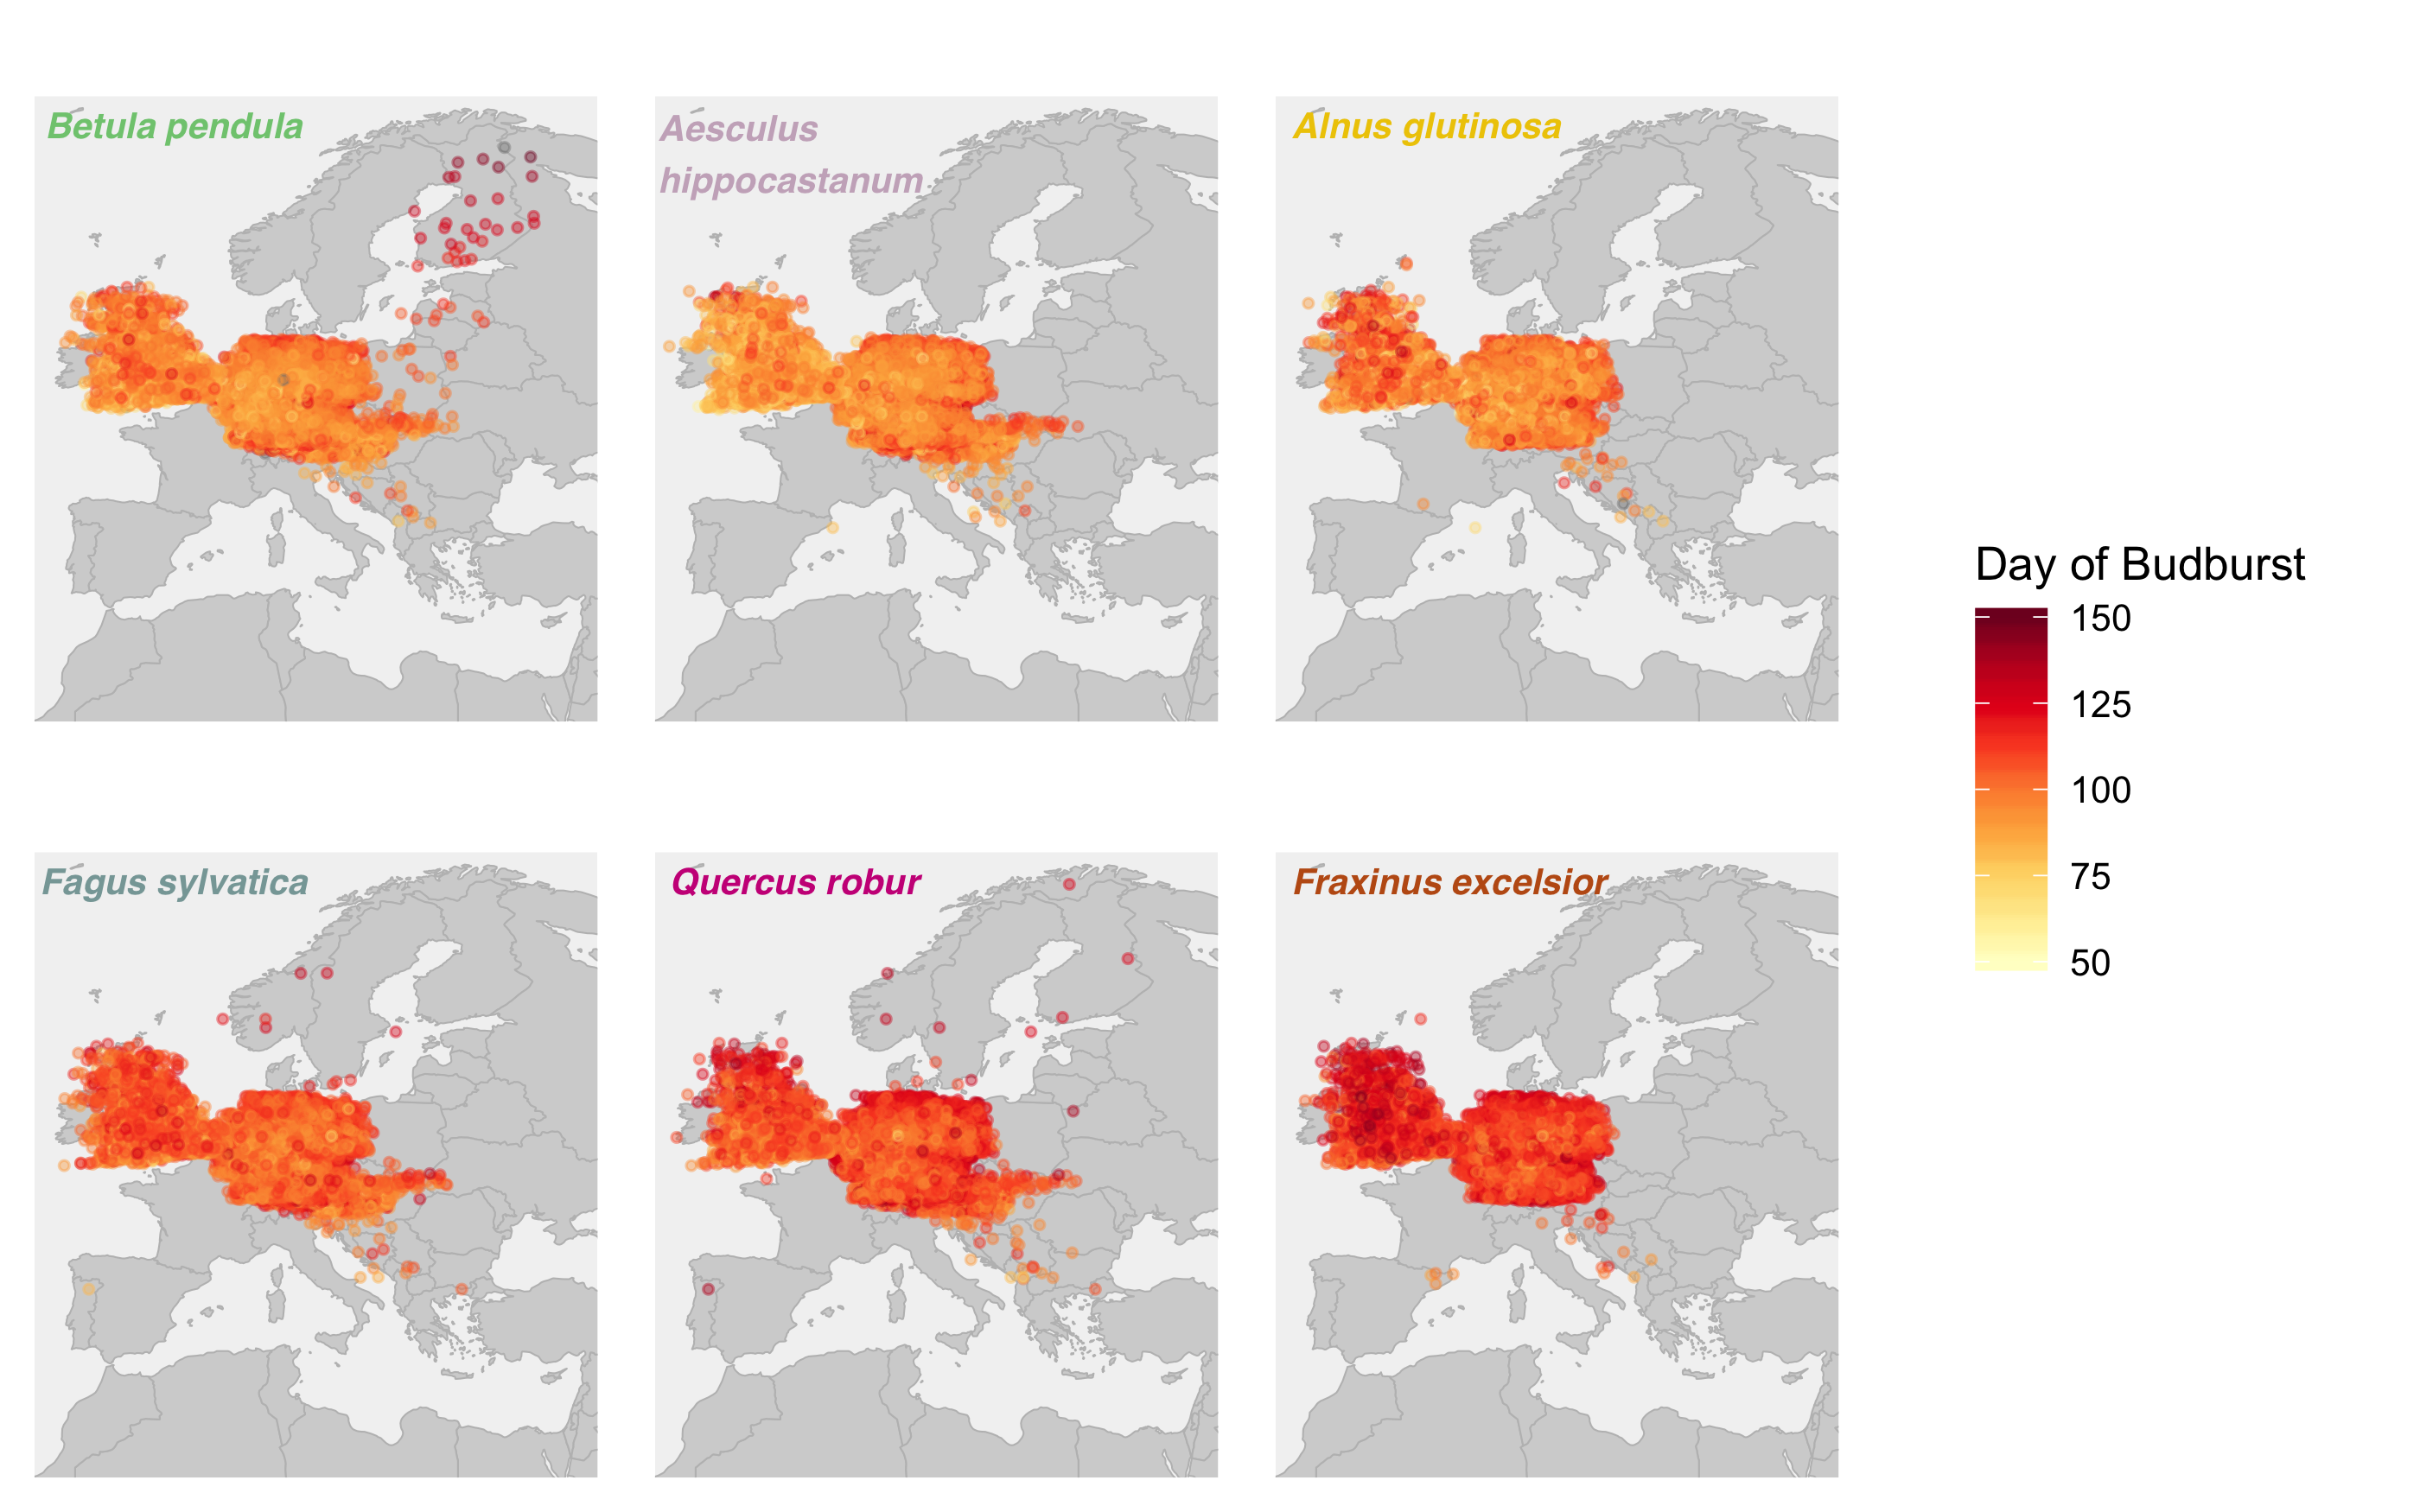
\includegraphics[width=14cm]{..//analyses/figures/BB_base.png}
  -\caption{The average day of budburst is mapped by site for each species. Species are ordered by day of budburst starting with \textit{Betula pendula} as the earliest budburst date to \textit{Fraxinus excelsior}. Earlier budburst dates are yellow and later budburst dates are in red. Species names are color-coded to match figures throughout the text. }\label{fig:bbmap}
  -\end{center}
  -\end{figure}}
  
{\begin{figure} [H]
  -\begin{center}
  -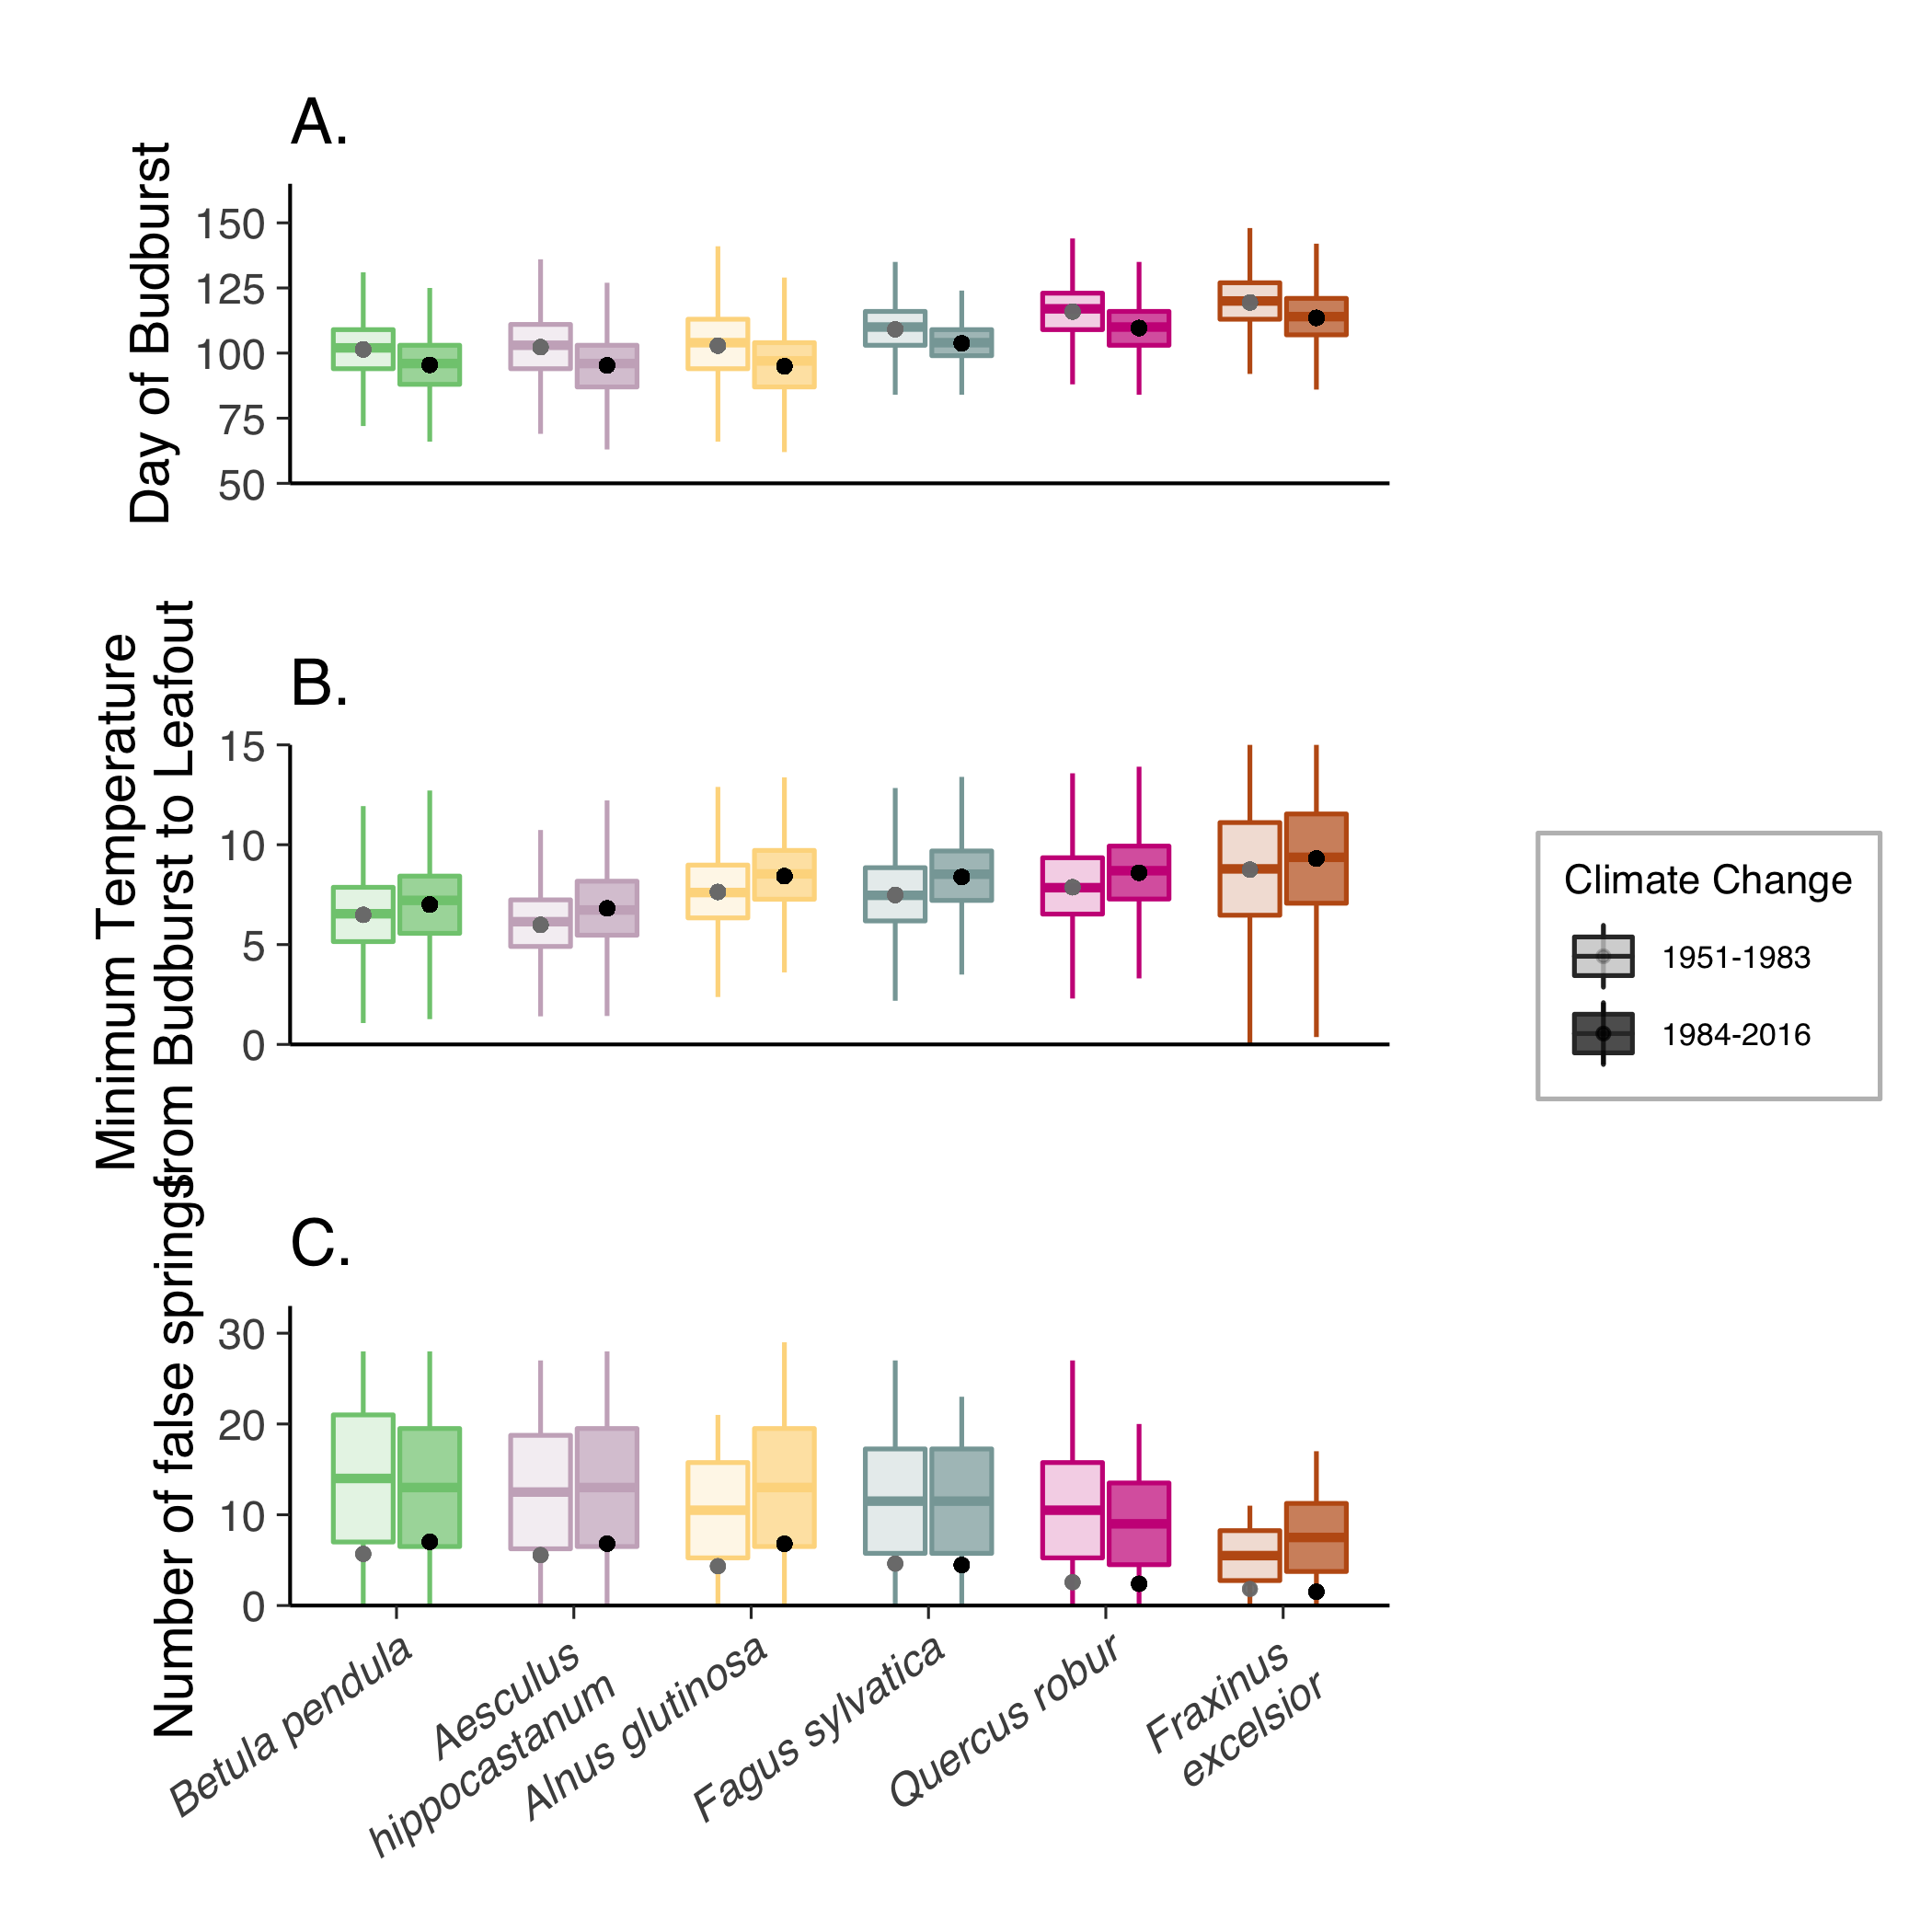
\includegraphics[width=14cm]{..//analyses/figures/Boxplot_BBTminFS_noDots_modests.png}
  -\caption{Budburst (A.), minimum temperatures between budburst and leafout (B.) and probability of false springs (C.) were compared before and after 1983 for each species across all sites. Dots and error bars overlaid on the box and whisker plots represent the simple model regression outputs (Tables S3-S5). Species are ordered by day of budburst and are color-coded to match the other figures.  }\label{fig:boxfs}
  -\end{center}
  -\end{figure}}
  
  
{\begin{figure} [H]
  -\begin{center}
  -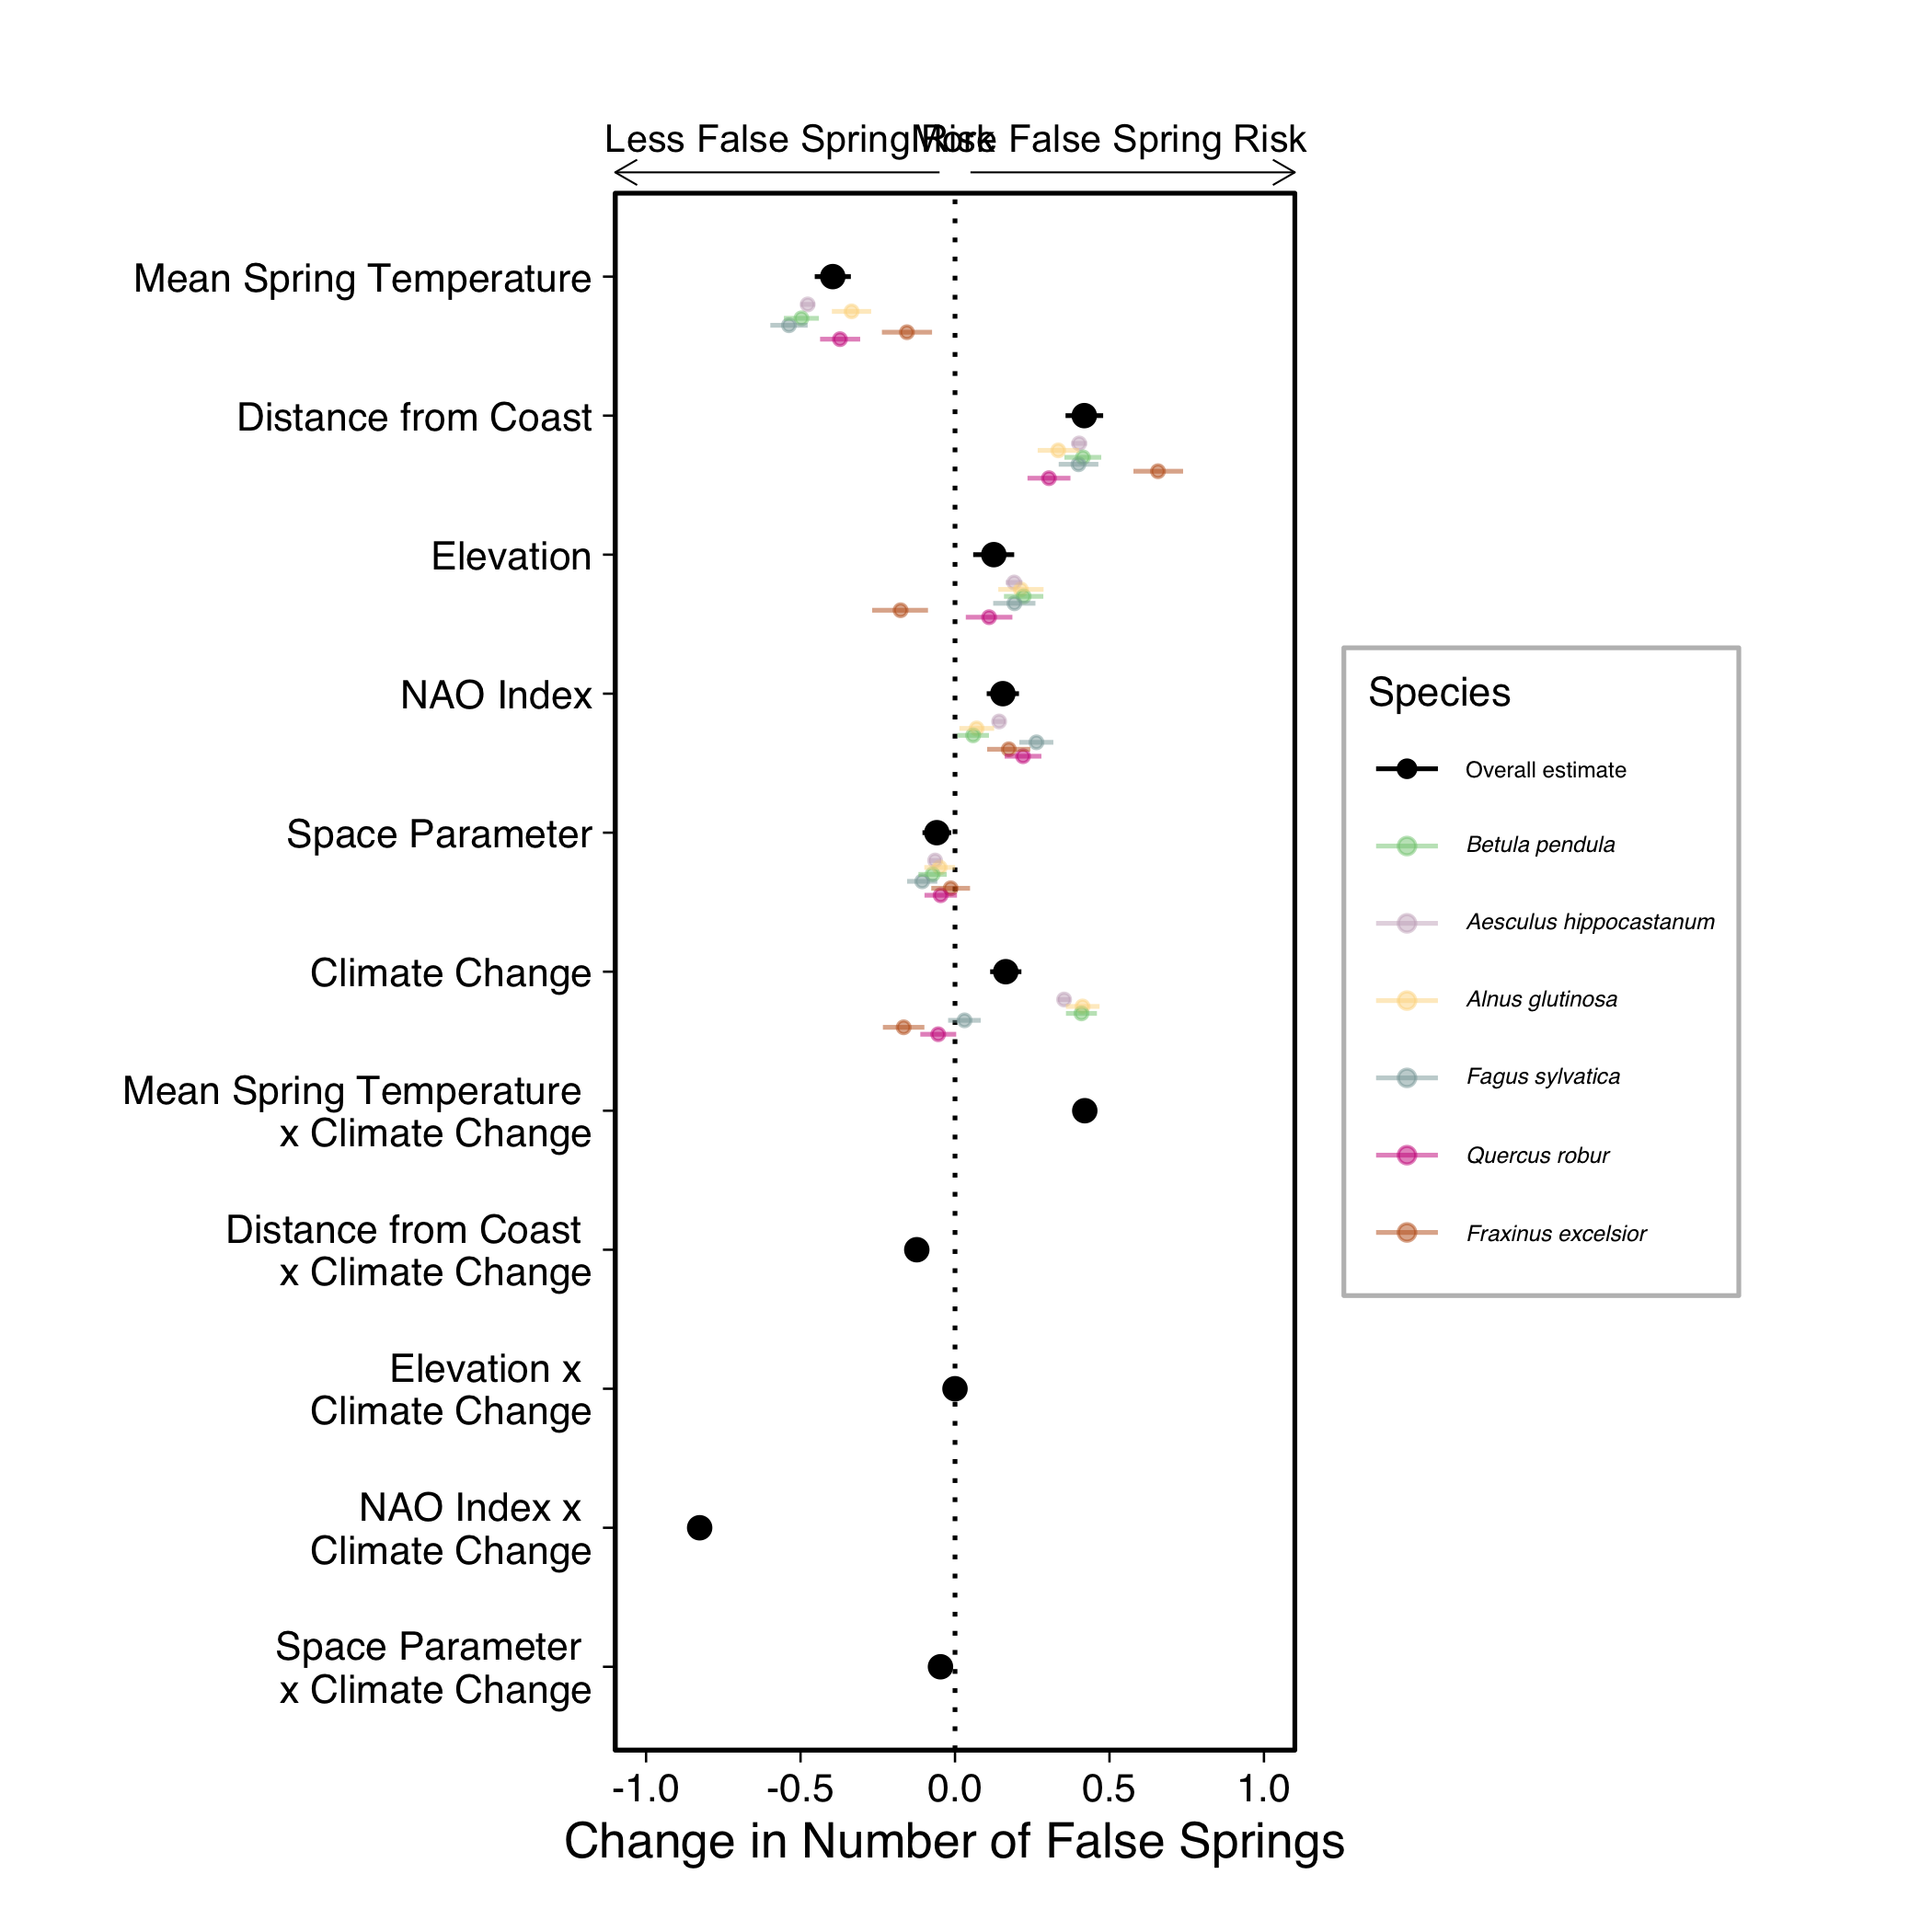
\includegraphics[width=12cm]{..//analyses/figures/model_output_90_origspp.png}
  -\caption{Effects of species, climatic and geographical predictors on false spring risk. More positive values indicate an increased probability of a false spring whereas more negative values suggest a lower probability of a false spring. Dots and lines show means and 90\% uncertainty intervals. Values closer to zero have less of an effect on false springs. There were 582,211 zeros and 172,877 ones for false springs in the data.}\label{fig:maineffects}
  -\end{center}
  -\end{figure}}


%{\begin{figure} [H]
 % -\begin{center}
  %-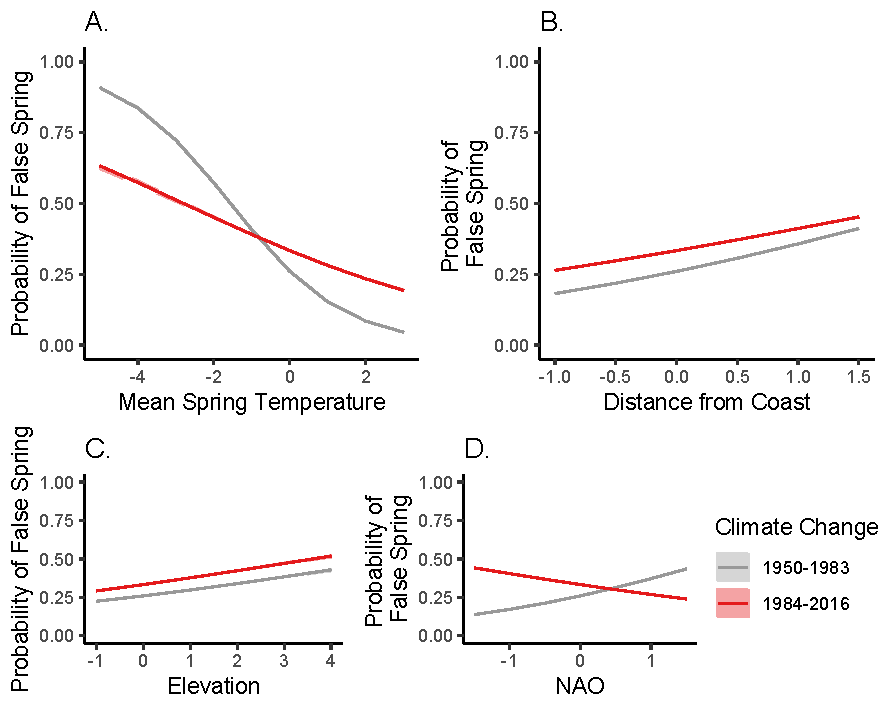
\includegraphics[width=16cm]{..//figures/InteractionPlots/IntrxnPlots_orig.pdf}
  %-\caption{Plots showing the interaction effects on false spring risk for each predictor coupled with climate change. (A.) As mean spring temperature increases, there were fewer false springs but there were fewer false springs after 1983 at sites with lower mean spring temperatures.  (B.) There were more false springs further from the coast and the rate of increase was consistent, however, there were fewer false springs in total after 1983. (C.) As elevation increased, false spring risk increased but the relationship remained consistent after 1983. (D.) As NAO indices increased, there were more false springs before 1983 but fewer after 1983. Since we found the z-score for each predictor, the x-axis for each panel does not reflect the raw data.}\label{fig:intrxns}
  %-\end{center}
  %-\end{figure}}
  
{\begin{figure} [H]
  -\begin{center}
  -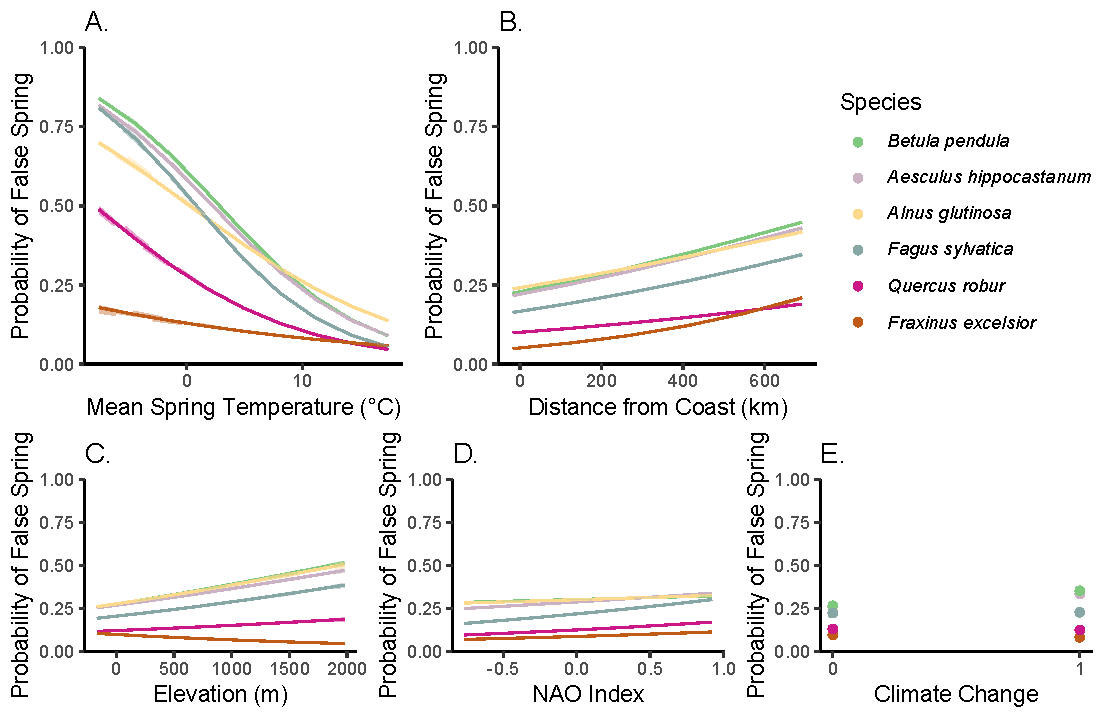
\includegraphics[width=16cm]{..//analyses/figures/InteractionPlots/Species_orig.pdf}
  -\caption{Species-level variation across geographic and spatial predictors (i.e., mean spring temperature (A.), distance from the coast (B.), elevation (C.), and NAO index (D.)). Lines and shading are the mean and 90\% uncertainty intervals for each species. To reflect the raw data, we converted the model output back to the original scale for the x-axis in each panel. }\label{fig:spp}
  -\end{center}
  -\end{figure}}


  



\end{document}
